\documentclass{article}
\usepackage{ctex}
\title{编译原理 期中试卷}
\author{} 
\date{}
\usepackage[a4paper,left=10mm,right=10mm,top=15mm,bottom=15mm]{geometry} 
\usepackage{graphicx} 
\usepackage{makecell}
\usepackage{tikz}
\begin{document}
\section*{一、不定项选择题}
\noindent
\textbf{1-5.}BCD\ AD\ CBD\ BD\ BD\\
\textbf{6-8.}ABCDEFH\ B\ A
\section*{二、填空题}
\noindent
\textbf{1.}T\ \{e,(,),+\}\ \{T,F\}\ (T+e),T+e,e\ e\\
\textbf{2.}$\{a^nb^mc^m\ |\ n\geq 0,m\geq 1\}$
\section*{三、}
\noindent
对于句子i+i-i,该文法有两种不同的推导:\\
$E\Rightarrow E+E\Rightarrow E+E-E\Rightarrow E+E-i\Rightarrow E+i-i\Rightarrow i+i-i$\\
$E\Rightarrow E-E\Rightarrow E+E-E\Rightarrow i+E-E\Rightarrow i+i-E\Rightarrow i+i-i$\\
因此该文法具有二义性,改写后的文法如下所示:\\
$E\rightarrow T\ |\ E+T\\
T\rightarrow F\ |\ T-F\\
F\rightarrow E\ |\ i$
\section*{四、}
\noindent
$¥((ndd\ |\ nd\ |\ n),(ddd,)^*ddd\ |\ ndd\ |\ nd \ |\ d).dd$
\section*{五、}
\noindent
对于串$(ba)^+(a^*b^*\ |\ a^*)$,构造NFA如下所示:\\
\begin{center}
    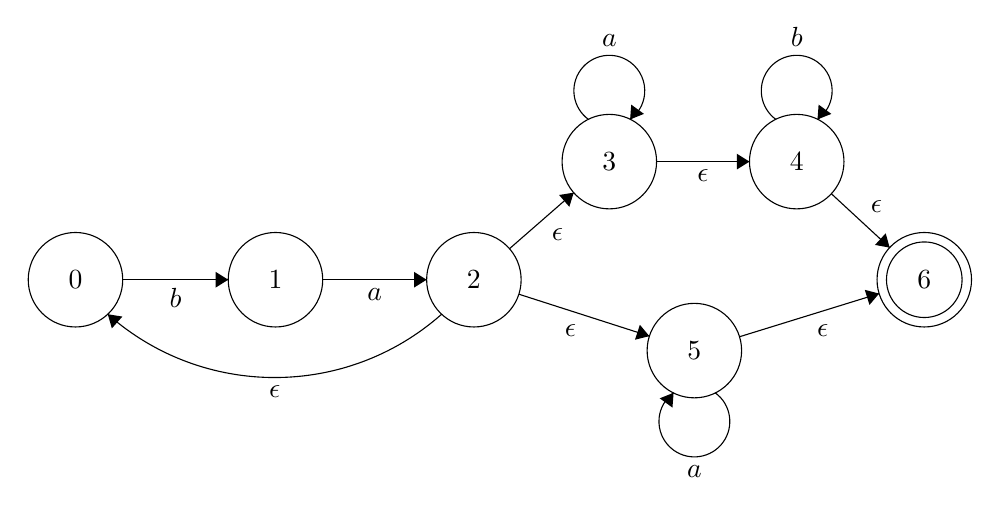
\begin{tikzpicture}[scale=0.2]
    \tikzstyle{every node}+=[inner sep=0pt]
    \draw [black] (6.4,-30.8) circle (3);
    \draw (6.4,-30.8) node {$0$};
    \draw [black] (19.1,-30.8) circle (3);
    \draw (19.1,-30.8) node {$1$};
    \draw [black] (31.7,-30.8) circle (3);
    \draw (31.7,-30.8) node {$2$};
    \draw [black] (40.3,-23.3) circle (3);
    \draw (40.3,-23.3) node {$3$};
    \draw [black] (52.2,-23.3) circle (3);
    \draw (52.2,-23.3) node {$4$};
    \draw [black] (45.7,-35.3) circle (3);
    \draw (45.7,-35.3) node {$5$};
    \draw [black] (60.3,-30.8) circle (3);
    \draw (60.3,-30.8) node {$6$};
    \draw [black] (60.3,-30.8) circle (2.4);
    \draw [black] (9.4,-30.8) -- (16.1,-30.8);
    \fill [black] (16.1,-30.8) -- (15.3,-30.3) -- (15.3,-31.3);
    \draw (12.75,-31.3) node [below] {$b$};
    \draw [black] (22.1,-30.8) -- (28.7,-30.8);
    \fill [black] (28.7,-30.8) -- (27.9,-30.3) -- (27.9,-31.3);
    \draw (25.4,-31.3) node [below] {$a$};
    \draw [black] (29.654,-32.988) arc (-48.44691:-131.55309:15.987);
    \fill [black] (8.45,-32.99) -- (8.71,-33.89) -- (9.38,-33.14);
    \draw (19.05,-37.51) node [below] {$\epsilon$};
    \draw [black] (34.56,-31.72) -- (42.84,-34.38);
    \fill [black] (42.84,-34.38) -- (42.24,-33.66) -- (41.93,-34.61);
    \draw (37.83,-33.59) node [below] {$\epsilon$};
    \draw [black] (47.023,-37.98) arc (54:-234:2.25);
    \draw (45.7,-42.55) node [below] {$a$};
    \fill [black] (44.38,-37.98) -- (43.5,-38.33) -- (44.31,-38.92);
    \draw [black] (33.96,-28.83) -- (38.04,-25.27);
    \fill [black] (38.04,-25.27) -- (37.11,-25.42) -- (37.76,-26.17);
    \draw (37.01,-27.54) node [below] {$\epsilon$};
    \draw [black] (43.3,-23.3) -- (49.2,-23.3);
    \fill [black] (49.2,-23.3) -- (48.4,-22.8) -- (48.4,-23.8);
    \draw (46.25,-23.8) node [below] {$\epsilon$};
    \draw [black] (38.977,-20.62) arc (234:-54:2.25);
    \draw (40.3,-16.05) node [above] {$a$};
    \fill [black] (41.62,-20.62) -- (42.5,-20.27) -- (41.69,-19.68);
    \draw [black] (50.877,-20.62) arc (234:-54:2.25);
    \draw (52.2,-16.05) node [above] {$b$};
    \fill [black] (53.52,-20.62) -- (54.4,-20.27) -- (53.59,-19.68);
    \draw [black] (54.4,-25.34) -- (58.1,-28.76);
    \fill [black] (58.1,-28.76) -- (57.85,-27.85) -- (57.17,-28.59);
    \draw (57.27,-26.56) node [above] {$\epsilon$};
    \draw [black] (48.57,-34.42) -- (57.43,-31.68);
    \fill [black] (57.43,-31.68) -- (56.52,-31.44) -- (56.82,-32.4);
    \draw (53.85,-33.6) node [below] {$\epsilon$};
    \end{tikzpicture}
\end{center}
使用子集法进行化简:\\ \\ \\ \\ \\ \\ \\ 
\begin{table}[h]
    \centering
\begin{tabular}{|p{5cm}<{\centering}|p{5cm}<{\centering}|p{5cm}<{\centering}|}   
    \hline
    \ & $I_a$ & $I_b$ \\
    \hline
    0 & $\Phi$ & 1 \\
    \hline
    1 & 0,2,3,4,5,6 & $\Phi$ \\
    \hline
    0,2,3,4,5,6 & 3,4,5,6 & 1,4,6 \\
    \hline
    1,4,6 & 0,2,3,4,5,6 & 4,6 \\
    \hline
    4,6 & $\Phi$ & 4,6 \\
    \hline
\end{tabular}
\end{table}
\\
改写后的状态转换表为:
\begin{table}[h]
    \centering
\begin{tabular}{|p{5cm}<{\centering}|p{5cm}<{\centering}|p{5cm}<{\centering}|}   
    \hline
    \ & $I_a$ & $I_b$ \\
    \hline
    0 & $\Phi$ & 1 \\
    \hline
    1 & 2 & $\Phi$ \\
    \hline
    2 & 3 & 4 \\
    \hline
    3 & 3 & 5 \\
    \hline
    5 & $\Phi$ & 5 \\
    \hline
\end{tabular}
\end{table}
\\
则确定化后以0为初态,以2,3,4,5为终态的DFA如下所示:
\begin{center}
    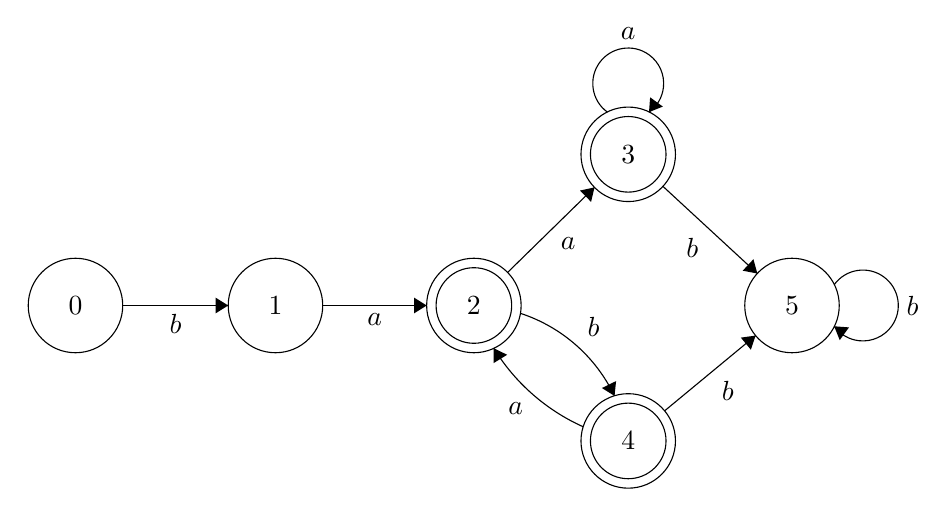
\begin{tikzpicture}[scale=0.2]
    \tikzstyle{every node}+=[inner sep=0pt]
    \draw [black] (6.4,-30.8) circle (3);
    \draw (6.4,-30.8) node {$0$};
    \draw [black] (19.1,-30.8) circle (3);
    \draw (19.1,-30.8) node {$1$};
    \draw [black] (31.7,-30.8) circle (3);
    \draw (31.7,-30.8) node {$2$};
    \draw [black] (31.7,-30.8) circle (2.4);
    \draw [black] (41.5,-39.4) circle (3);
    \draw (41.5,-39.4) node {$4$};
    \draw [black] (41.5,-39.4) circle (2.4);
    \draw [black] (41.5,-21.2) circle (3);
    \draw (41.5,-21.2) node {$3$};
    \draw [black] (41.5,-21.2) circle (2.4);
    \draw [black] (51.9,-30.8) circle (3);
    \draw (51.9,-30.8) node {$5$};
    \draw [black] (9.4,-30.8) -- (16.1,-30.8);
    \fill [black] (16.1,-30.8) -- (15.3,-30.3) -- (15.3,-31.3);
    \draw (12.75,-31.3) node [below] {$b$};
    \draw [black] (22.1,-30.8) -- (28.7,-30.8);
    \fill [black] (28.7,-30.8) -- (27.9,-30.3) -- (27.9,-31.3);
    \draw (25.4,-31.3) node [below] {$a$};
    \draw [black] (34.648,-31.296) arc (71.93664:25.52615:10.093);
    \fill [black] (40.63,-36.54) -- (40.73,-35.6) -- (39.83,-36.04);
    \draw (39.3,-32.82) node [above] {$b$};
    \draw [black] (38.645,-38.503) arc (-114.14213:-148.39508:12.839);
    \fill [black] (32.96,-33.51) -- (32.95,-34.46) -- (33.81,-33.93);
    \draw (34.35,-36.93) node [below] {$a$};
    \draw [black] (33.84,-28.7) -- (39.36,-23.3);
    \fill [black] (39.36,-23.3) -- (38.44,-23.5) -- (39.14,-24.22);
    \draw (37.69,-26.48) node [below] {$a$};
    \draw [black] (40.177,-18.52) arc (234:-54:2.25);
    \draw (41.5,-13.95) node [above] {$a$};
    \fill [black] (42.82,-18.52) -- (43.7,-18.17) -- (42.89,-17.58);
    \draw [black] (43.7,-23.23) -- (49.7,-28.77);
    \fill [black] (49.7,-28.77) -- (49.45,-27.86) -- (48.77,-28.59);
    \draw (45.57,-26.49) node [below] {$b$};
    \draw [black] (54.58,-29.477) arc (144:-144:2.25);
    \draw (59.15,-30.8) node [right] {$b$};
    \fill [black] (54.58,-32.12) -- (54.93,-33) -- (55.52,-32.19);
    \draw [black] (43.81,-37.49) -- (49.59,-32.71);
    \fill [black] (49.59,-32.71) -- (48.65,-32.84) -- (49.29,-33.61);
    \draw (47.83,-35.59) node [below] {$b$};
    \end{tikzpicture}
    \end{center}
经检验,这一DFA无法进行简化.\\    
对于串$(ba)^*ba^+(b^*\ |\ \epsilon)$,构造NFA如下所示:\\
\begin{center}
    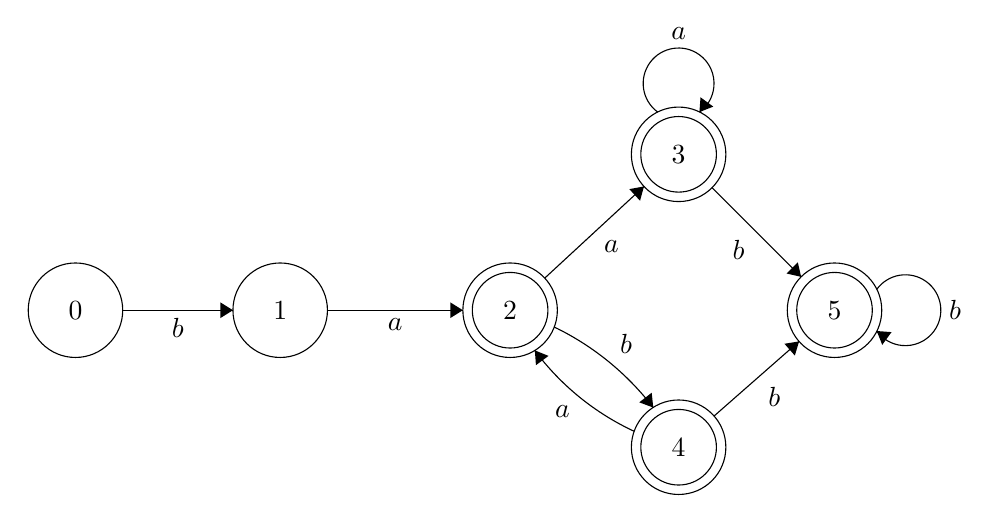
\begin{tikzpicture}[scale=0.2]
    \tikzstyle{every node}+=[inner sep=0pt]
    \draw [black] (6.4,-30.8) circle (3);
    \draw (6.4,-30.8) node {$0$};
    \draw [black] (19.4,-30.8) circle (3);
    \draw (19.4,-30.8) node {$1$};
    \draw [black] (34,-30.8) circle (3);
    \draw (34,-30.8) node {$2$};
    \draw [black] (34,-30.8) circle (2.4);
    \draw [black] (44.7,-20.9) circle (3);
    \draw (44.7,-20.9) node {$3$};
    \draw [black] (44.7,-20.9) circle (2.4);
    \draw [black] (44.7,-39.5) circle (3);
    \draw (44.7,-39.5) node {$4$};
    \draw [black] (44.7,-39.5) circle (2.4);
    \draw [black] (54.6,-30.8) circle (3);
    \draw (54.6,-30.8) node {$5$};
    \draw [black] (54.6,-30.8) circle (2.4);
    \draw [black] (9.4,-30.8) -- (16.4,-30.8);
    \fill [black] (16.4,-30.8) -- (15.6,-30.3) -- (15.6,-31.3);
    \draw (12.9,-31.3) node [below] {$b$};
    \draw [black] (22.4,-30.8) -- (31,-30.8);
    \fill [black] (31,-30.8) -- (30.2,-30.3) -- (30.2,-31.3);
    \draw (26.7,-31.3) node [below] {$a$};
    \draw [black] (43.377,-18.22) arc (234:-54:2.25);
    \draw (44.7,-13.65) node [above] {$a$};
    \fill [black] (46.02,-18.22) -- (46.9,-17.87) -- (46.09,-17.28);
    \draw [black] (57.28,-29.477) arc (144:-144:2.25);
    \draw (61.85,-30.8) node [right] {$b$};
    \fill [black] (57.28,-32.12) -- (57.63,-33) -- (58.22,-32.19);
    \draw [black] (46.95,-37.52) -- (52.35,-32.78);
    \fill [black] (52.35,-32.78) -- (51.42,-32.93) -- (52.08,-33.68);
    \draw (50.78,-35.64) node [below] {$b$};
    \draw [black] (41.88,-38.489) arc (-114.91319:-143.31483:16.587);
    \fill [black] (35.57,-33.35) -- (35.64,-34.29) -- (36.44,-33.7);
    \draw (37.33,-36.81) node [below] {$a$};
    \draw [black] (36.8,-31.866) arc (64.25393:37.51804:17.517);
    \fill [black] (43.09,-36.98) -- (42.99,-36.04) -- (42.2,-36.65);
    \draw (41.37,-33.56) node [above] {$b$};
    \draw [black] (36.2,-28.76) -- (42.5,-22.94);
    \fill [black] (42.5,-22.94) -- (41.57,-23.11) -- (42.25,-23.85);
    \draw (40.43,-26.34) node [below] {$a$};
    \draw [black] (46.82,-23.02) -- (52.48,-28.68);
    \fill [black] (52.48,-28.68) -- (52.27,-27.76) -- (51.56,-28.47);
    \draw (48.51,-26.33) node [below] {$b$};
    \end{tikzpicture}
    \end{center}
使用子集法进行化简:\\ \\ \\ \\ \\ \\ \\
\begin{table}[h]
    \centering
\begin{tabular}{|p{5cm}<{\centering}|p{5cm}<{\centering}|p{5cm}<{\centering}|}   
    \hline
    \ & $I_a$ & $I_b$ \\
    \hline
    0,2 & $\Phi$ & 1,3 \\
    \hline
    1,3 & 0,2,3,4,5,6 & $\Phi$ \\
    \hline
    0,2,3,4,5,6 & 3,4,5,6 & 1,3,5,6 \\
    \hline
    3,4,5,6 & 0,2,3,4,5,6 & 5,6 \\
    \hline
    5,6 & $\Phi$ & 5,6 \\
    \hline
\end{tabular}
\end{table}
\\
改写后的状态转换表为:
\begin{table}[h]
    \centering
\begin{tabular}{|p{5cm}<{\centering}|p{5cm}<{\centering}|p{5cm}<{\centering}|}   
    \hline
    \ & $I_a$ & $I_b$ \\
    \hline
    0 & $\Phi$ & 1 \\
    \hline
    1 & 2 & $\Phi$ \\
    \hline
    2 & 3 & 4 \\
    \hline
    3 & 3 & 5 \\
    \hline
    5 & $\Phi$ & 5 \\
    \hline
\end{tabular}
\end{table}
\\
则确定化后以0为初态,以2,3,4,5为终态的DFA如下所示:
\begin{center}
    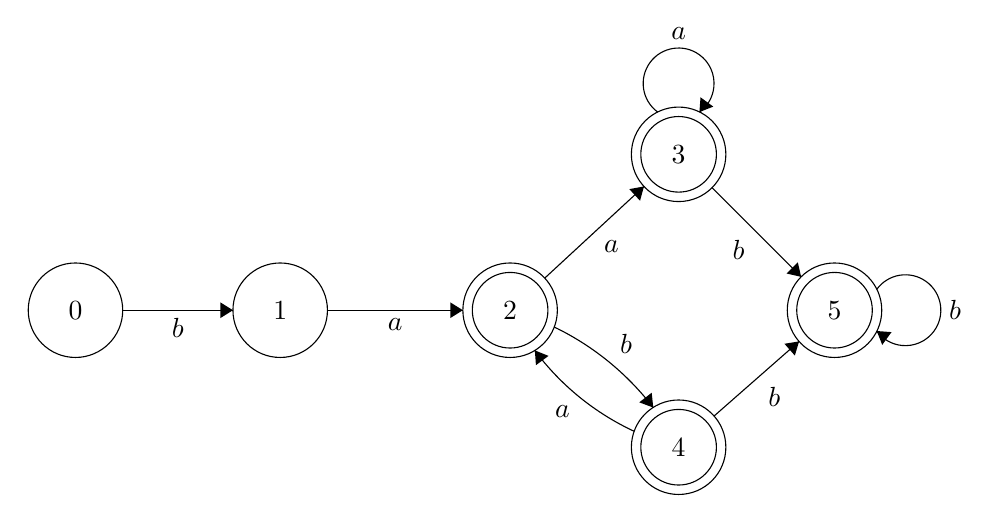
\begin{tikzpicture}[scale=0.2]
    \tikzstyle{every node}+=[inner sep=0pt]
    \draw [black] (6.4,-30.8) circle (3);
    \draw (6.4,-30.8) node {$0$};
    \draw [black] (19.4,-30.8) circle (3);
    \draw (19.4,-30.8) node {$1$};
    \draw [black] (34,-30.8) circle (3);
    \draw (34,-30.8) node {$2$};
    \draw [black] (34,-30.8) circle (2.4);
    \draw [black] (44.7,-20.9) circle (3);
    \draw (44.7,-20.9) node {$3$};
    \draw [black] (44.7,-20.9) circle (2.4);
    \draw [black] (44.7,-39.5) circle (3);
    \draw (44.7,-39.5) node {$4$};
    \draw [black] (44.7,-39.5) circle (2.4);
    \draw [black] (54.6,-30.8) circle (3);
    \draw (54.6,-30.8) node {$5$};
    \draw [black] (54.6,-30.8) circle (2.4);
    \draw [black] (9.4,-30.8) -- (16.4,-30.8);
    \fill [black] (16.4,-30.8) -- (15.6,-30.3) -- (15.6,-31.3);
    \draw (12.9,-31.3) node [below] {$b$};
    \draw [black] (22.4,-30.8) -- (31,-30.8);
    \fill [black] (31,-30.8) -- (30.2,-30.3) -- (30.2,-31.3);
    \draw (26.7,-31.3) node [below] {$a$};
    \draw [black] (43.377,-18.22) arc (234:-54:2.25);
    \draw (44.7,-13.65) node [above] {$a$};
    \fill [black] (46.02,-18.22) -- (46.9,-17.87) -- (46.09,-17.28);
    \draw [black] (57.28,-29.477) arc (144:-144:2.25);
    \draw (61.85,-30.8) node [right] {$b$};
    \fill [black] (57.28,-32.12) -- (57.63,-33) -- (58.22,-32.19);
    \draw [black] (46.95,-37.52) -- (52.35,-32.78);
    \fill [black] (52.35,-32.78) -- (51.42,-32.93) -- (52.08,-33.68);
    \draw (50.78,-35.64) node [below] {$b$};
    \draw [black] (41.88,-38.489) arc (-114.91319:-143.31483:16.587);
    \fill [black] (35.57,-33.35) -- (35.64,-34.29) -- (36.44,-33.7);
    \draw (37.33,-36.81) node [below] {$a$};
    \draw [black] (36.8,-31.866) arc (64.25393:37.51804:17.517);
    \fill [black] (43.09,-36.98) -- (42.99,-36.04) -- (42.2,-36.65);
    \draw (41.37,-33.56) node [above] {$b$};
    \draw [black] (36.2,-28.76) -- (42.5,-22.94);
    \fill [black] (42.5,-22.94) -- (41.57,-23.11) -- (42.25,-23.85);
    \draw (40.43,-26.34) node [below] {$a$};
    \draw [black] (46.82,-23.02) -- (52.48,-28.68);
    \fill [black] (52.48,-28.68) -- (52.27,-27.76) -- (51.56,-28.47);
    \draw (48.51,-26.33) node [below] {$b$};
    \end{tikzpicture}
    \end{center}
经检验,这一DFA无法进行简化.\\    
观察两个DFA可知,题目中给出的正规式等价.
\section*{六、}
\noindent
\textbf{(1)}消除左递归后的文法如下所示:\\
$S\rightarrow a\ |\ \^{}\ |\ (T)$\\
$T\rightarrow ST'$\\
$T'\rightarrow \epsilon\ |\ ,ST'$\\
首先,由于已经消除左递归,该文法必然不含左递归.\\
考察各非终结符的产生式,有$FIRST(a)$、$FIRST(\^{})$、$FIRST(T)$两两不相交,\\
$FIRST(\epsilon)\cap FIRST(,ST')=\Phi$.\\
又有$FIRST(T')\cap FOLLOW(T')=\Phi$.\\
综上所述,该文法为LL(1)文法.\\
\textbf{(2)}
\begin{table}[h]
    \centering
\begin{tabular}{|p{2cm}<{\centering}|p{2cm}<{\centering}|p{2cm}<{\centering}|p{2cm}<{\centering}|p{2cm}<{\centering}|p{2cm}<{\centering}|p{2cm}<{\centering}|}   
    \hline
    \ & a & $\^{}$ & ( & ) & , & \# \\
    \hline
    S & S$\rightarrow$a & S$\rightarrow\^{}$ & S$\rightarrow$(T) & \ & \ & \ \\
    \hline
    T & T$\rightarrow$ST' & T$\rightarrow$ST' & T$\rightarrow$ST' & & & \\
    \hline
    T' & & & & T'$\rightarrow\epsilon$& T'$\rightarrow$,ST' & \\
    \hline
\end{tabular}
\end{table}
\\
\textbf{(3)}
\begin{tabbing}
    \hspace{1.5cm} \= \hspace{3cm}\= \hspace{3cm}\= \hspace{3cm}\= \kill
    \textbf{步骤}\>\textbf{符号栈}\>\textbf{输入串}\>\textbf{所用产生式}\\
    0\>\#S\>(a,a)\#\\
    1\>\#)T(\>(a,a)\#\>$S\rightarrow(T)$\\
    2\>\#)T\>a,a)\#\\
    3\>\#)T'S\>a,a)\#\>$T\rightarrow ST'$\\
    4\>\#)T'a\>a,a)\#\>$S\rightarrow a$\\
    5\>\#)T'\>,a)\#\\
    6\>\#)T'S,\>,a)\#\>$T'\rightarrow ST'$\\
    7\>\#)T'S\>a)\#\\
    8\>\#)T'a\>a)\#\>$S\rightarrow a$\\
    9\>\#)T'\>)\#\\
    10\>\#)\>)\#\> $T'\rightarrow\epsilon$\\
    11\>\#\>\#
\end{tabbing}
因此,该串是文法G的句子.
\section*{七、}
\noindent
\textbf{(1)}原文法的拓广文法如下所示:\\$S\rightarrow A\\
A\rightarrow BaBb\\ A\rightarrow DbDa \\ B\rightarrow\epsilon\\ 
D\rightarrow\epsilon$\\
构造LR(1)项目集族得:\\
$I_0=\{[S\rightarrow\cdot A,\#],[A\rightarrow\cdot BaBb,\#],[A\rightarrow\cdot DbDa,\#],[B\rightarrow\cdot,a],[D\rightarrow\cdot,b]\}\\
I_1=GOTO(I_0,A)=\{[S\rightarrow A\cdot,\#]\}\\
I_2=GOTO(I_0,B)=\{[A\rightarrow B\cdot aBb,\#]\}\\
I_3=GOTO(I_0,D)=\{[A\rightarrow D\cdot bDa,\#]\}\\
I_4=GOTO(I_2,a)=\{[A\rightarrow Ba\cdot Bb,\#],[B\rightarrow\cdot,b]\}\\
I_5=GOTO(I_3,b)=\{[A\rightarrow Db\cdot Da,\#],[D\rightarrow\cdot,a]\}\\
I_6=GOTO(I_4,B)=\{[A\rightarrow BaB\cdot b,\#]\}\\
I_7=GOTO(I_5,D)=\{[A\rightarrow DbD\cdot a,\#]\}\\
I_8=GOTO(I_6,b)=\{[A\rightarrow BaBb\cdot,\#]\}\\
I_9=GOTO(I_7,a)=\{[A\rightarrow DbDa\cdot,\#]\}$\\
对于$I_0$,存在规约-规约冲突,$[B\rightarrow\cdot,a],[D\rightarrow\cdot,b]$,而$FOLLOW(B)\cap FOLLOW(D)\neq\Phi$,故不能用SLR(1)方式解决冲突,
然而这两个状态的展望符不同,因此可以用LR(1)方式解决冲突.\\
综上所述,该文法是LR(1)文法但不是SLR(1)文法.\\
\textbf{(2)}
\begin{table}[h]
    \centering
\begin{tabular}{|p{2cm}<{\centering}|p{2cm}<{\centering}|p{2cm}<{\centering}|p{2cm}<{\centering}|p{2cm}<{\centering}|p{2cm}<{\centering}|p{2cm}<{\centering}|}   
    \hline
    \ & a & b & \# & B & D & A \\
    \hline
    $I_0$ & $r_3$ & $r_4$ && 2 & 3 & 1\\
    \hline
    $I_1$ && acc &&&& \\
    \hline
    $I_2$ & $s_4$ &&&&& \\
    \hline
    $I_3$ && $s_5$ &&&& \\
    \hline
    $I_4$ && $r_3$ && 6 && \\
    \hline 
    $I_5$ && $r_4$ &&& 7 & \\
    \hline
    $I_6$ && $s_8$ &&&& \\
    \hline
    $I_7$ & $s_9$ &&&&& \\
    \hline
    $I_8$ &&& $r_2$ &&& \\
    \hline
    $I_9$ &&& $r_3$ &&& \\
    \hline
\end{tabular}
\end{table}
\end{document}
